%% Begin slides template file
\documentclass[11pt,t,usepdftitle=false,aspectratio=169]{beamer}
%% ------------------------------------------------------------------
%% - aspectratio=43: Set paper aspect ratio to 4:3.
%% - aspectratio=169: Set paper aspect ratio to 16:9.
%% ------------------------------------------------------------------

\usetheme[nototalframenumber,foot,logo]{uibk}

\title[Segfault Slayer]{Progress Update 3: Segfault Slayer}

\author[Schmölz Lukas, Schöpf Emanuel, Schweigl Dominik]{\textbf{Schmölz Lukas}, Schöpf Emanuel, Schweigl Dominik}

\headerimage{3}

\begin{document}

\section{Bookmark Title}
\subsection{Overview}


\begin{frame}
    \frametitle{Game Overview}

    \textbf{Game Idea:}
    \begin{itemize}
        \item Metroidvania-style 2D side-scroller
        \item Player fights programming concepts and bugs (mainly C++ related)
        \item Playful, Pixel-theme (e.g. ASCII-Art for textures)
    \end{itemize}

    \bigskip

    \textbf{World Design:}
    \begin{itemize}
        \item First Area: Hardware with Logic Operators
        \item Second Area: Programming with loops and other concepts
    \end{itemize}
\end{frame}


\begin{frame}{Previous Goals}
    \vspace{1em}
    \begin{itemize}
        \item Player/Enemy Health System
        \item More Enemies / Boss
        \item Keyboard Binding Management
        \item Entity spawns in the Map
        \item Game Saves
    \end{itemize}
\end{frame}


\begin{frame}{Audio Manager}
    \begin{columns}[T]
        \begin{column}{0.55\textwidth}
            \small
            \textbf{Centralized Audio Playback}
            \begin{itemize}
                \item Singleton \texttt{AudioManager} owns every sound and music
                \item constructed in similar fashion to \texttt{AssetManager}
                \item Buffers loaded once, lazily, on first use
                \item Master sound \& music volume split - can be adjusted independently
                \item Global pause / resume / stop wired into pause menu
            \end{itemize}
        \end{column}

        \begin{column}{0.4\textwidth}
            \vspace{1.5em}
            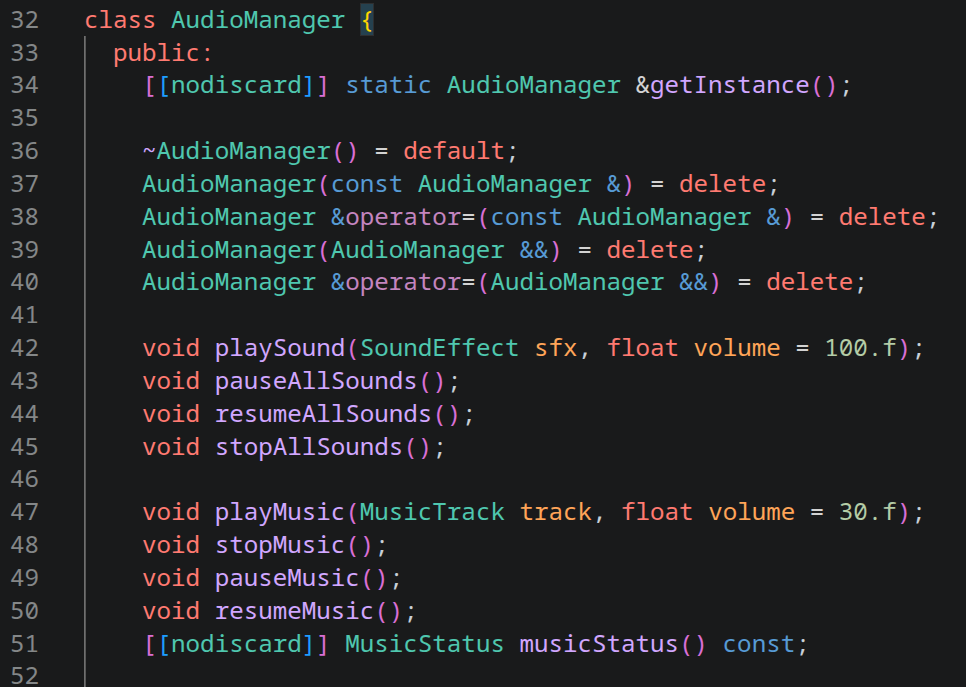
\includegraphics[width=\linewidth]{_images/audio_manager.png}
        \end{column}
    \end{columns}
\end{frame}


\begin{frame}{User Ability}
    \begin{columns}[T]

        \begin{column}{0.4\textwidth}
            \small
            \textbf{Wall Jump}
            
            \begin{itemize}
                \item Allows player to slide and jump from walls
                \item Key part in reaching second game area
                \item Obtainable from defeating first boss
            \end{itemize}

        \end{column}

        \begin{column}{0.5\textwidth}
            \centering
            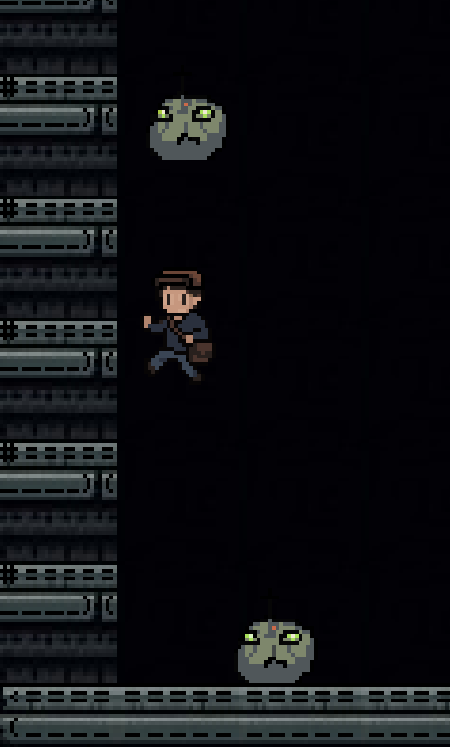
\includegraphics[width=0.4\linewidth]{_images/wall_jump1.png}
            \hfill
            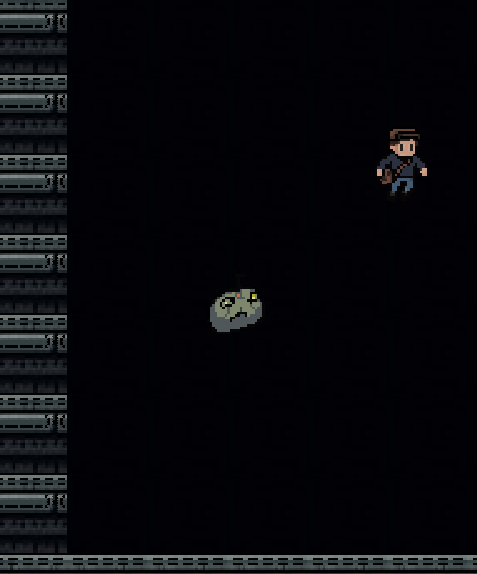
\includegraphics[width=0.55\linewidth]{_images/wall_jump2.png}
        \end{column}

    \end{columns}
\end{frame}


\begin{frame}{Menus, Menus, Menus}

\vspace{1.5em}

\begin{columns}[c]
    \column{0.33\textwidth}
    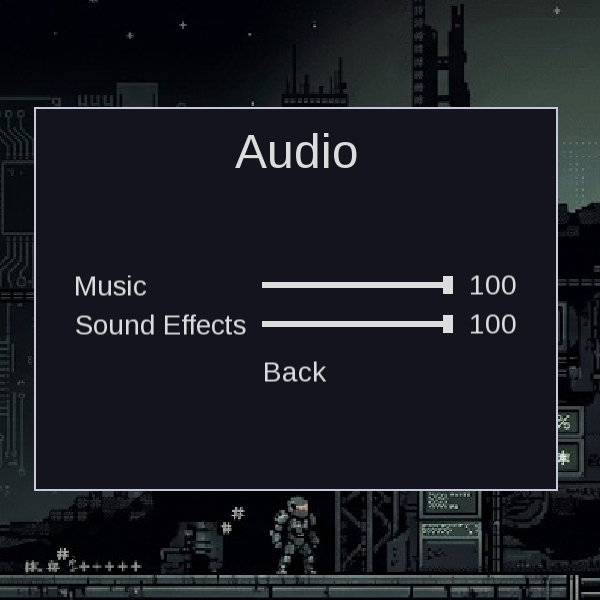
\includegraphics[width=\linewidth]{_images/audio_menu.png}

    \column{0.33\textwidth}
    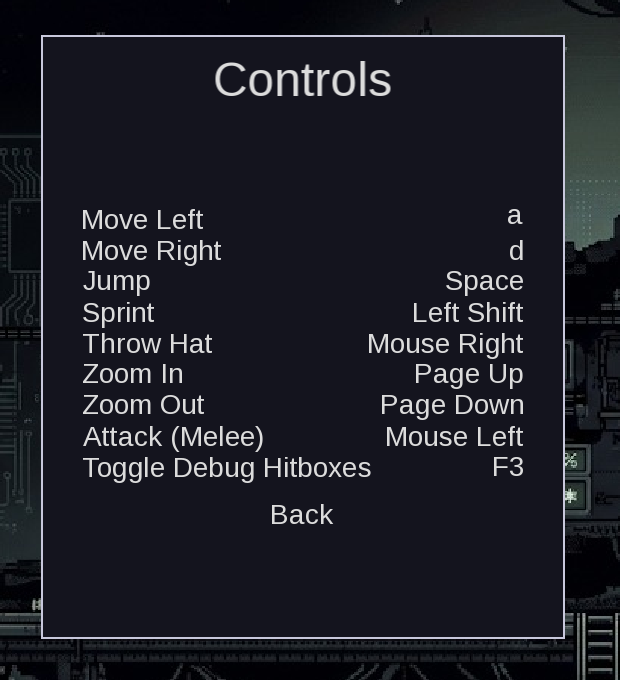
\includegraphics[width=\linewidth]{_images/controls_menu.png}

    \column{0.33\textwidth}
    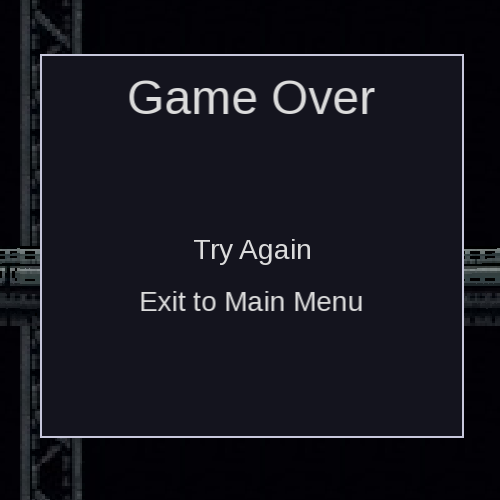
\includegraphics[width=\linewidth]{_images/game_over_menu.png}
\end{columns}

\end{frame}


\begin{frame}{Combat System}
    \begin{columns}[T]
        \begin{column}{0.5\textwidth}
            \vspace{3em}
            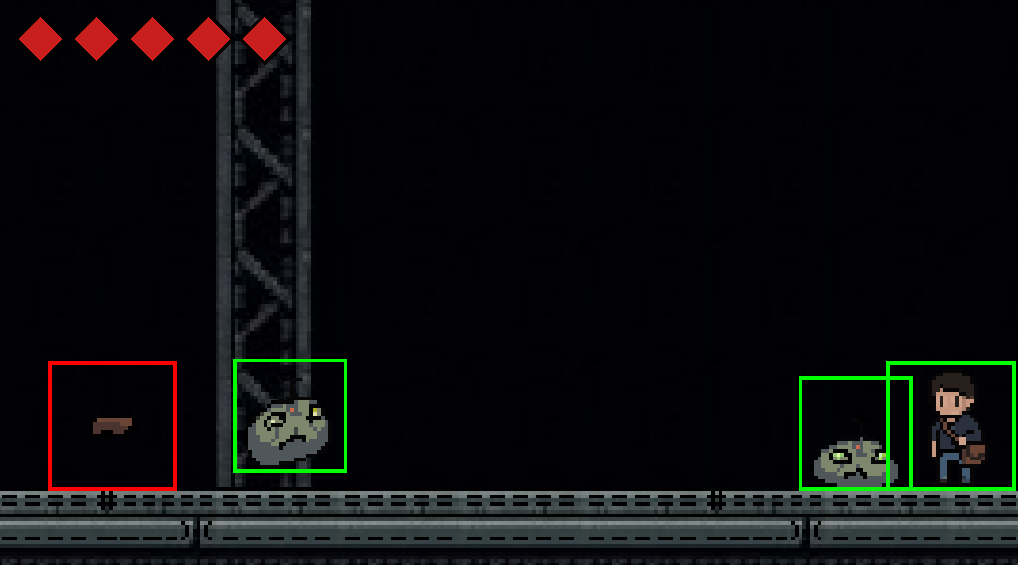
\includegraphics[width=\linewidth]{_images/combat_system.png}
        \end{column}
    
        \begin{column}{0.55\textwidth}
            \small
            \textbf{Overlap and Damage Resolver}
            \begin{itemize}
                \item Entities publish \texttt{Hitbox} / \texttt{Hurtbox} rectangles each frame
                \item \texttt{GameScene} collects them and sends them to \texttt{CombatSystem}
                \item Central \texttt{CombatSystem} resolves every hitbox against every opposing-team hurtbox
                \item Each attack gets a \texttt{sourceId} - one (source, victim) pair damages at most once across all its active frames
                \item Invulnerable hurtboxes are skipped (i-frames during knockback)
            \end{itemize}

        \end{column}


    \end{columns}
\end{frame}


\begin{frame}{Combat System Mechanics}
    \begin{columns}[T]
        \begin{column}{0.55\textwidth}
        
        \begin{itemize}
            \item\textbf{Knockback}\\
            Entites get short velocity boost in opposite direction of received hit.
    
            \vspace{1em}
            
            \item\textbf{Hurt-Flash}\\
            Short red sprite coloring on taking damage.
    
            \vspace{1em}
    
            \item\textbf{i-Frames}\\
            Short invincibility time when boxes first overlap. Allows for more fluid game feel.
        \end{itemize}
        
        \end{column}

        \begin{column}{0.4\textwidth}
            \begin{flushright}
                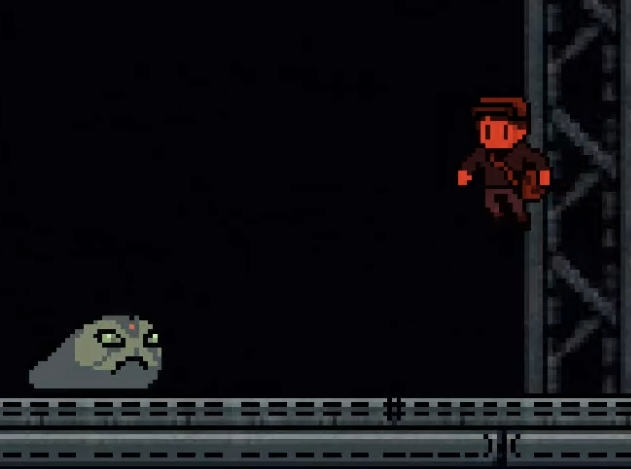
\includegraphics[width=\linewidth]{_images/knockback.png}
            \end{flushright}
        \end{column}
    \end{columns}
\end{frame}


\begin{frame}[plain,c]
    \begin{center}
        \Huge{Demo \& Code Review}
    \end{center}
\end{frame}

\begin{frame}{Next Steps}
    \vspace{1em}
    \begin{itemize}
        \item More Enemies / Boss
        \item Inventory and State Menu
        \item Obtainable Player Abilities
        \item Map Expansion (Entity Spawns, Teleport Tiles, Collectables)
        \item Game Saves
    \end{itemize}
\end{frame}

\end{document}
